\documentclass[11pt]{beamer}
\usetheme{Warsaw}
\usepackage[utf8]{inputenc}
\usepackage{natbib}
\usepackage{amsmath}
\usepackage{graphicx}
\usepackage{subcaption}
\usepackage{tikz}


\title{UE COM}
\subtitle{Learning Deep CNN Denoiser Prior for Image Restoration}
\author{Adrien Zabban}
\date{8 janvier 2024}

\begin{document}

\maketitle

% --- Probleme ---
\begin{frame}{Le Probleme inverse}
    \begin{block}{But}
        On a une image observée dégradée $y$ et l'on veut retrouver l'image d'origine $x$. On sait 
        que cette image a été dégradée de la façon suivante : 
        $$y = Hx + v$$
        où $H$ est la matrice de 
        dégradation que l'on connait, et $v$ est un bruit gaussien d'écart-type $\sigma$ inconnue.
    \end{block}
    \begin{figure}[b]
        \centering
        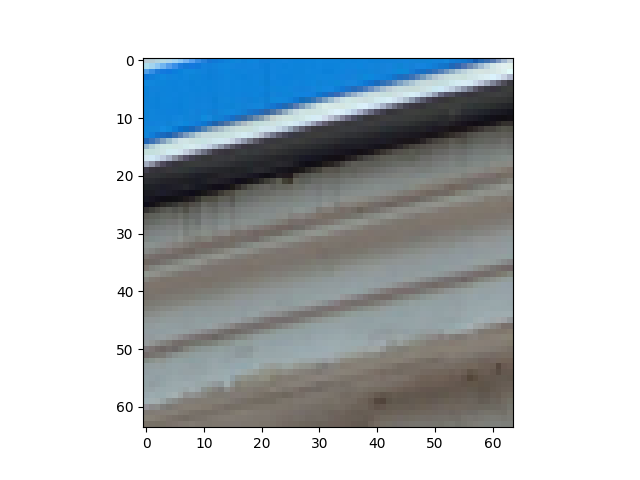
\includegraphics[width=0.41\textwidth]{../debluring/x.png}
        \begin{tikzpicture}[overlay, remember picture]
            \draw[->, blue, very thick] (0,1.5) -- (1,1.5) node[midway, above, blue] {$f_{H, \sigma}$};
        \end{tikzpicture}
        \hspace{1cm}
        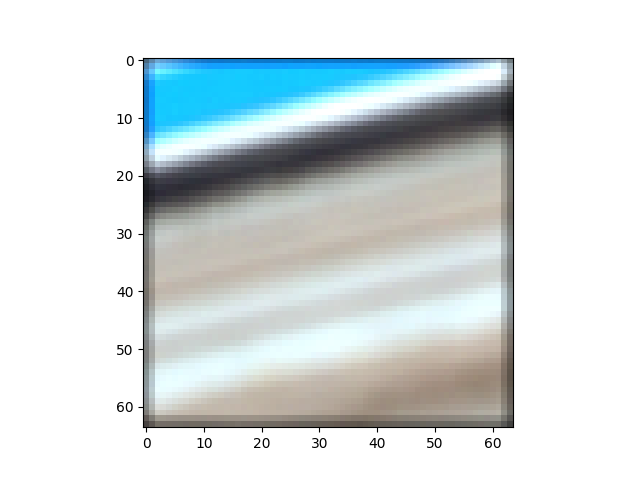
\includegraphics[width=0.41\textwidth]{../debluring/y.png}
        \caption{image d'orignine x (à gauche) et l'image dégradée y (à droite).}
    \end{figure}
\end{frame}


\begin{frame}{Maximiser la log likelihood}
    \begin{visibleenv}<1->
        \begin{align*}
            \max_x \log(p(x|y)) &= \max_x \log(p(x, y)) \quad \text{car } p(x|y) = p(x, y) \times p(y) \\
            &= \max_x \log(p(y|x)) + \log(p(x)) \\
            &\quad \text{or } (y|x) = (v+Hx|x) \sim \mathcal{N}(Hx, \sigma^2) \\
            &= \max_x -\frac{\lVert y-Hx \rVert ^2}{2 \sigma^2} + \log(p(x)) \\
            &= \min_x \frac{1}{2}\lVert y-Hx \rVert ^2 + \lambda \Phi(x) \quad \text{avec } \Phi = -\frac{\log \circ p}{\lambda}
        \end{align*}
    \end{visibleenv}

    \begin{visibleenv}<2->
        \begin{alertblock}{But}
            On veut donc trouver $\hat{x}$ tel que: $\hat{x} = \text{arg} \min_x \frac{1}{2} \lVert y-Hx \rVert ^2 + \lambda \Phi(x)$
        \end{alertblock}
    \end{visibleenv}
\end{frame}

\begin{frame}{Une première méthode: ISTA}
    raconter ISTA
\end{frame}

\begin{frame}{Une deuxième méthode: Half Quadratic Splitting (HQS)}
    \begin{visibleenv}<1->
        \begin{exampleblock}{Idée}
            Diviser la variable $x$ pour découpler le terme de fidélité et le terme de régularisation.
        \end{exampleblock}
    \end{visibleenv}
    \begin{visibleenv}<2->
        On a l'équivalence entre:
        $$ \min_x \frac{1}{2}\lVert y-Hx \rVert^2 + \lambda \Phi(x) $$
        $$ \Leftrightarrow \min_{x, z} \frac{1}{2}\lVert y-Hx \rVert ^2 + \lambda \Phi(z) \quad \text{tel que} \quad  z=x$$
        En rajoutant un parametre $\mu$:
        $$ \Leftrightarrow \min_{x, z, \mu}  \frac{1}{2}\lVert y-Hx \rVert ^2+\lambda \Phi(z) + \frac{\mu}{2}\lVert z-x \rVert ^2 $$
        On appele $\mathcal{L}_{\mu}(x,z)$, le terme que l'on doit minimizer.
    \end{visibleenv}
\end{frame}

\begin{frame}{Une deuxième méthode: Half Quadratic Splitting (HQS)}
    Comme $\mathcal{L}_{\mu}(x,z)$ est décroissante (pour les variable $x$ et $z$), on a:
    $$\min_{x, z} \mathcal{L}_{\mu}(x,z) = \lim_{k \rightarrow \infty} \min_z \min_x \min_z \dots \min_x \mathcal{L}_{\mu}(x,z)$$
    On peut alors écrire:
    \begin{equation*}
        \left\{
        \begin{aligned}
            & \arg \min_x \quad \lVert y - Hx \rVert^2 + \mu \lVert z - x \rVert^2 \\
            & \arg \min_z \quad \frac{\mu}{2}\lVert z - x \rVert^2 + \lambda \Phi(z)
        \end{aligned}
        \right.
    \end{equation*}
\end{frame}


\begin{frame}{Les systèmes de plug and play}
    en quoi ça consiste
\end{frame}

\begin{frame}{Le Denoiser}
    le model
\end{frame}

\begin{frame}{Le Denoiser}
    train et inférance
\end{frame}

\begin{frame}{Plug and play}
    résultats
\end{frame}



\end{document}
